\documentclass[12pt]{article}

\usepackage{graphicx}
\usepackage[margin=1in]{geometry}
\usepackage{setspace}
\usepackage[backend=biber]{biblatex}

\addbibresource[location=remote]{http://127.0.0.1:23119/better-bibtex/export?/library;id:1/collection;key:GT493ARA/Thesis.biblatex}

\title{Thesis}
\author{Tom Zurales}
\date{July 2025}

\begin{document}
\doublespace

\maketitle

\newpage

\begin{abstract}
  This research details the implementation and analysis of a novel, viewpoint aware method for map point culling for use in keypoint based visual SLAM systems. This method makes use of perspective dependent shells around each map point, allowing for the storage of overall observability metadata using constant additional space. This metadata allows for the overall probability of a point's existence to be continuously calculated using a simple Bayesian update step. This existence probability can be used in a myriad of ways. This research explores its use as a method of culling outdated map points, such as those originally seen on an object which has since moved, and as an extension to the RANSAC algorithm, providing the ability to select more robust map points. We provide the implementation of the perspective aware metadata shell as an open-source library, as well as an ORB\_SLAM3 implementation utilizing the library for point culling and RANSAC improvement. Additionally, a set of co-registered visual-inertial-lidar datasets are released, containing scenarios specifically intended to exercise and characterize the performance of the system. Through our analysis, (discuss effects on well known, non-dynamic SLAM datasets, along with my datasets)
\end{abstract}

\newpage

\tableofcontents

\section{Introduction}

The research presented in this thesis details the conception, implementation and analysis of a novel viewpoint aware probability model for the existence of map points in 

\subsection{Motivation}

The inspiration for this research came from a project to utilize keypoint based visual SLAM on the Astrobee robots on the International Space Station (ISS). At the time of the project, Astrobee navigation was accomplished through localization on a pre-generated map, which required both astronaut and ground team intervention to produce \cite{soussanAstroLocEfficientRobust2022}. Due to the tight schedules and high costs associated with ISS astronaut work, this map creation happened very rarely.

The ISS is a challenging place to perform robot navigation tasks. The primary structure of the station remains the same, with nodes always connecting to the same nodes, but regular resupply, hardware replacement, temporary experimental setups, and general crew living can cause the station to gradually change from day to day. This high variation in the internal features of the space station caused the Astrobee maps to quickly go out of date, severely limiting the robot's autonomous capabilities and utilities as a research platform \cite{PLACEHOLDER}.

It was the intention of the project to run keypoint based visual SLAM on board the Astrobees, allowing them the capabilities to create and update their own maps and eliminating the need for astronaut intervention. In order to be useful for ISS operations, the SLAM algorithm had to output its map and localization estimates in the established ISS coordinate frame \cite{PLACEHOLDER}. To accomplish this, the decision was made early on to build off of a SLAM system which included the ability to load and merge previously generated maps. Assuming the system localizes in the pregenerated map, the coordinate frame can be preserved between mapping runs by merging the new data into the old map. This is where the non-static nature of the ISS produces problems for SLAM. If a map is generated a significant time before it is used, there is ample opportunity for the visual features of the environment to change, leading to poor performance when attempting to localize within this previously generated map. While out of scope for the previous project, the researchers noted that these out of date visual features in the previously generated map posed a challenge for SLAM operations in similarly dynamic environments.

\subsubsection{Problem Statement}

A primary assumption in SLAM is that the environment remains static throughout operations. It is obvious 

\subsubsection{Research Questions}

Does a probability model which identifies and culls outdated map points provide significant improvements to relocalization and tracking during map reuse in keypoint-based SLAM?
To what extent do dynamic changes in a map affect mapping and relocalization performance?
Can this be used as a heuristic to determine when to re-enable mapping on MAVs?

The spacial understanding provided by SLAM is not only useful, but necessary for systems intending to operate in and interact with physical environments. Virtual reality, robotics, and industrial automation all make use of SLAM to generate an internal map of the local and global environments. SLAM does have the distinction of being a "solved" problem in the ideal case. If an agent is able to perfectly measure the environment, and is guaranteed to make correct data associations, then a perfect map can be generated and the agent's location within that map can be known with certainty. This ideal case makes several assumptions, paramount of which is the existence of ideal sensors, but there is a secondary assumption that the state of the world does not change.

It is obvious that the assumption of a static, unchanging world does not hold in practice. In fact, the inspiration for this research came from attempts to perform localization on the International Space Station (ISS). As of the time of publication, there are three mobile autonomous vehicles (MAVs) on board the ISS known as Astrobees. While used for numerous experiments and product development tasks on the ISS, the Astrobees are prone to failure due to loss of localization. The primary cause of this localization failure is the constant changes occurring on the ISS, including equipment changes, resupply missions, and any other activities which may change the visual features of the ISS.

The situation on the ISS is not unique, and would be experienced by any agent running SLAM in all but the most tightly controlled environments. VR goggles using use SLAM to determine their position in 3D space within a room must contend with new objects which are placed in the room, the changing images shown on the TV, people walking in and out of view, etc. Robots operating in an office environment must be robust to moved desks, the movement of people, and more. Even robotic operations in an unmanned space station (a situation proposed for the Lunar Gateway project) would need to be able to perform despite changing lighting conditions, moved equipment, other MAVs in view, etc. Overall, a requirement that a SLAM agent gets to operate in a pristine, unchanging environment would be an insurmountable barrier for real world use.

The field of research into making SLAM perform over long timeframes has been called lifetime SLAM[], eluding to the fact that SLAM systems with the requirement for an unchanging environment will still be able to operate successfully over short timeframes, but will struggle with missions which take place over multiple days, weeks, months, or years.

This research is specific to a subset of the greater SLAM problem known as keypoint-based, visual SLAM. The distinctions between these will be discussed in detail in the Background section, but a high-level overview is offered here. Keypoint-based visual SLAM operates on images taken over time. The core principal involves constructing a sparse 3D map of image features which are identifiable from multiple perspectives. This is accomplished through photogrammetry methods such as the 5-point method, which allows the depths of 5 matched pairs of points, and the parallax transformation to be determined from two 2d images [FACT CHECK and CITATION].

<!-- Go into a few more details about some of the other fields of research which are used by SLAM -->

There are numerous keypoint-based visual SLAM implementations seeing use today, but all follow a relatively straightforward pipeline, defined as follows:

1. Determine an initial set of 3D points from two images with sufficient parallax
2. For subsequent images, match features with previously identified 3D points
3. Determine the transformation between the previous image and the new image which maximizes the number of map point alignments

Implementation differences tend to come from optimization steps, pruning of redundant data, anomaly handling, and additional sensor integrations. In order to achieve lifetime SLAM, the system must be able to determine what data is remaining static, what data is changing, and act accordingly. Imagine an art gallery with many paintings on the walls. If you were to visit this gallery on two separate occasions one year apart, the paintings on the walls may change, but you are able to identify that you are in the same gallery. People perform this contextual elimination of data which may change on a subconscious level []. Replicating this contextual awareness in SLAM allows systems to recognize and focus on unchanging data while ignoring dynamic data which could clutter and confuse the agent's internal map.

The benefits of eliminating data which is not helpful for long-term operations are plentiful. Just like culling redundant data, culling dynamic data reduces the overall size of the map. This reduces storage capacity requirements, while providing a smaller pool of data through which processes like Random Sample Consensus (RanSaC) need to search. A keypoint which was seen on an object which is later moved will always be an outlier in subsequent observations. Through culling of these dynamic data points, we can improve the speed and robustness of the several optimization steps, reduce overall system hardware requirements, and increase confidence in the accuracy and validity of the produced maps.

Numerous methods for improving SLAM's performance over long timeframes have been implemented, pushing the field of SLAM to the point where it is now seeing deployment in numerous dynamic environments. A discussion of several of these implementations takes place in the Background section, with a focus on each implementation's strengths, weaknesses, and overall effectiveness. An area that remains lacking is implementations on MAVs with limited compute. Due to their mobile nature, MAVs are inherently compute limited, as any additional weight and power consumption decreases capability and operation time. This prevents the inclusion of many popular models for dynamic data elimination such as image segmentation and semantic identification. Other methods utilizing statistical methods for point existence exist, but fail to fully utilize the vast array of data to update their predictions

\subsection{Objectives and Scope}

This research intends to build upon the previously developed probability models, in order to distill the update step of each map point's probability of existence into a simple Bayesian update step. The goals for this model are as follows:

1. To utilize constant additional space for each map point
2. To complete the update step in constant time
3. To resist updating confidence levels with redundant data

\subsection{Contribution}

Through this research, we introduce an incrementally updated directional confidence model for the existence of map points. This model differs from other point removal optimizations in several ways. First, this implementation avoids the use of neural networks, facilitating use on resource constrained hardware without facilities optimized to run them. Second, while other probability based point removal optimizations have been developed, this model introduces the idea of utilizing a continuously updated perspective dependent shell of metadata for each keypoint, which can be used to reduce the problem of point existence to a simple Bayesian update step. This implementation allows perspective of observation to play a role in the point's existence probability update step, and avoids some of the common a priori work such as prior estimation common to other point removal optimization techniques. This shell is implemented in both finite and continuous modalities, utilizing regular convex polyhedral shells in the finite case, and von-meiser fisher distributions on the sphere in the continuous case.

To facilitate future research, this model is released as an open-source library, which is compatible with any keypoint based visual SLAM implementation. Additionally, a collection of co-registered visual-inertial and LIDAR datasets is provided, containing instances of multiple traversals through the same environments with changes to scene contents. Information regarding the locations of these environmental changes is included in the dataset, facilitating the benchmarking of point removal optimization implementations.

\subsection{Road Map}

Chapter X of this thesis discusses the background of the general SLAM problem, covering the history, use cases, and general pipeline utilized by SLAM systems. This is followed by a deeper dive into keypoint-based visual SLAM, the sensor modality targeted by this research. We provide a brief survey of widely utilized extensions to the core SLAM algorithm which target deficiencies in the core pipeline. Finally, we discuss fields outside the scope of SLAM which provide insight and methodology into this research.

Chapter X discusses works related to this research, specifically focusing on extensions targeting improved performance in dynamic situations, with additional focus given to those methods which utilize point removal optimizations.

\section{Background}
\label{sec:background}

In this chapter, we provide a high level overview of SLAM, with special focus paid to the Keypoint-Based Visual SLAM modality and the ORB-SLAM3 implementation. This research uses ideas from the field of Directional Statistics, so an overview of the subject and the Von-Mises Fisher distribution is provided.

\subsection{Keypoint-Based Visual SLAM}
\label{sec:kv_slam_background}

Keypoint-Based Visual SLAM is a subset of the wider SLAM ecosystem characterized by the use of cameras as the primary sensor, and image features (keypoints) extracted from 

\begin{figure}[!ht]
    \centering
    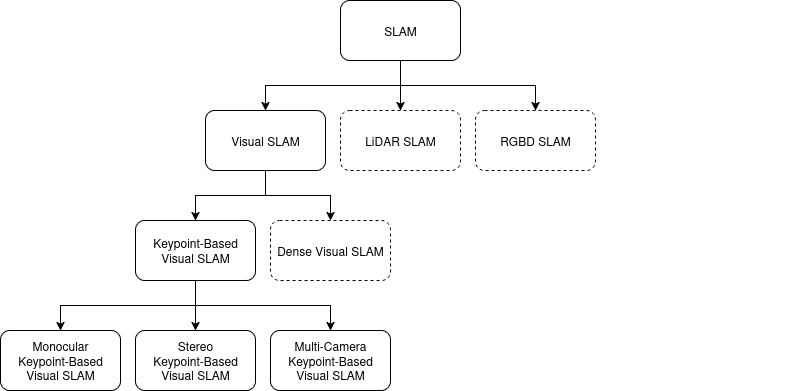
\includegraphics[width=0.8\textwidth]{resources/slam_family_tree.png}
    \caption{Keypoint-based Visual SLM pipeline showing the flow of data from sensor input to map and pose output.}
    \label{fig:slam_family_tree}
\end{figure}

% What is SLAM? What are its goals? What are its use cases?
SLAM refers to the joint problem of simultaneously generating a map of an environment and estimating the position of an observer within that map based on sensor observations. With research beginning in the 1980s \cite{smithEstimatingUncertainSpatial1988}, SLAM has become a de facto standard in robotics for tasks which require operations within unfamiliar environments. The benefit of SLAM when compared to other navigation methods such as pure localization is the ability to operate with no a-prioiri information, instead creating and incrementally updating the map at runtime. The selection of sensors is extremely flexible, with many popular implementations existing for camera, LIDAR, and RGBD based sensor modalities. Through careful selection of sensors, SLAM systems can operate in a wide variety of environments, from indoor office spaces to densely forested areas, and even underwater or in space.  These features make SLAM a powerful too for autonomous navigation, leading to its widespread use in robotics, augmented reality, and autonomous vehicles.

% What are the defining characteristics of keypoint based visual SLAM as opposed to other SLAM methods?
This research targets Keypoint-Based Visual SLAM (KV-SLAM), a specific modality of SLAM characterized by its use of one or more cameras as the primary sensor, and the use of keypoints as opposed to raw pixel values as the primary data for constructing the map and performing localization. As opposed to other sensor modalities such as LIDAR and RGBD, which take direct 3D measurements of the environment, KV-SLAM relies on the principles of epipolar geometry to infer depth and camera motion from the relative position of keypoints between image frames. The map generated by a KV-SLAM system is a sparse point cloud of 3D map points. Core to this research is the concept of the keypoint, map point, and sparse map, motivating a discussion on the definitions and structure of these types, and how they relate to the larger KV-SLAM pipeline.


% Describe the structure of a map in kvSKAM, including keyframes, map points, and their relationships.
The primary input to a KV-SLAM system is the keypoint. A keypoint is the combination of an image feature and a descriptor. Image features can take many forms, but for the purposes of SLAM, they should be identifiable, meaning they are quick to compute, and differentiable, meaning they are unique enough to tell one instance of a feature from another. Image features are differentiated using a descriptor, which is a vector representation of the feature that captures its unique characteristics. Ideally, keypoints should be invariant to changes in scale, rotation, and illumination, allowing them to be reliably matched between images taken from different viewpoints or under different lighting conditions.

Map points represent the extrapolation of keypoints into 3D space. Two views of the same set of keypoints can be used to triangulate the 3D position of the visual feature, in conjunction with the camera transformation between the two views. Depending on the implementation, map points often store additional metadata, such as the set frames in which they were observed, the descriptors of the keypoints they were derived from, etc. The primary contribution of this research is a novel method of determining and representing the observability of map points at the individual point level, allowing for the efficient and accurate identification of outdated map points.

The sparse map is the collection of all map points, acting as a 3D representation of the environment. It is used to localize new frames by finding a transformation that aligns the currently seen keypoints with the existing map points. This 2D-3D alignment is accomplished through an optimization process which iteratively refines the camera transform to minimize the reprojection error between the matched features.

% Explain how data flows through a keypoint-based visual SLAM system, from sensor input to map and pose output.
With these structures in hand, we can describe the pipeline which data follows through a generic KV-SLAM system. A graphical representation of the pipeline can be seen in Figure \ref{fig:kv_slam_pipeline}, each stage is expanded on here.

1. Initialization

\begin{figure}[!ht]
    \centering
    % \includegraphics[width=0.8\textwidth]{figures/kv_slam_pipeline}
    \caption{Keypoint-based Visual SLAM pipeline showing the flow of data from sensor input to map and pose output.}
    \label{fig:kv_slam_pipeline}
\end{figure}

% High level overview of the challenges of SLAM: computational complexity, sensor error accumulation, dynamic environments
This high-level overview of KV-SLAM Despite numerous advancements, the computational complexity of performing SLAM in real-time remains a challenge, meaning that on many resource constrained platforms, implementations can struggle to keep up with the rate of sensor data acquisition \cite{semenovaQuantitativeAnalysisSystem2022}. Additionally, because there is no fixed reference, SLAM systems can suffer from sensor error accumulation, leading to inaccurate maps and poses over time \cite{cadenaPresentFutureSimultaneous2016}. These issues are compounded as the timeframe, scale, and environmental dynamics of the SLAM task increase. Larger environments require larger, more complex maps, which produce higher computational load and longer processing times. Dynamic environments, where objects can move or change either during the SLAM process or between runs, are a particular challenge, as most SLAM systems tend to operate best in static environments, and can struggle to maintain accurate pose estimation and map consistence in the presence of moving objects. The field of SLAM research known as \textit{lifelong SLAM} \cite{cadenaPresentFutureSimultaneous2016} focuses on addressing these challenges, and will be covered in detail in Section \ref{sec:related_work}.


\subsection{ORB-SLAM3}

ORB-SLAM3 is a KV-SLAM implementation which is popular in research contexts due to its performance

\subsubsection{Loop Closure}
\subsubsection{Relocalization}
\subsubsection{Map Reuse}
\subsubsection{Map Point Culling}
\subsection{The Von Mises-Fisher Distribution}

This work uses the von Mises-Fisher distribution, a probability distribution defined on the unit sphere, as the basis for the viewpoint-a

\section{Related Work}
\label{sec:related_work}

This chapter contextualizes this thesis within the broader body of SLAM research. The topics discussed are selected for their relevance to two previously outlined objectives: the identification and removal of data that could cause instability, and the improvement of SLAM performance over long time horizons. While the goals of this research align with the topics of semantic rejection and lifelong SLAM, the methods applied are more closely related to change detection, point stability and re-observability confidence. The following sections explore the key ideas from these topics, and relate them to the proposed research.

\subsection{Change Detection}

In the context of SLAM, change detection refers to the identification of discrepancies between the map and the environment. In lifelong SLAM operations, change detection is often used to assist with map maintenance tasks by identifying areas of change and updating them to match the current environment. However, change detection has been used for many other purposes. Change detection methods can be split based on the abstraction level at which they operate.

\subparagraph{Object Level}
Larsen et al. \cite{larsenChangeDetectionModel} utilized pairs of images to identify geometric inconsistencies in existing 3D maps, allowing for the identification of individual added or removed objects.

\subparagraph{}

\subsection{Lifelong SLAM}

The term Lifelong SLAM has varied definitions throughout the literature, but common themes of robustness to dynamic change, and long-term operation can be seen. For simplicity, this research adopts the definition provided by Shi et al. \cite{shiAreWeReady2020}, describing lifelong SLAM as the ability for a robot to generate, maintain, and localize within a map of a particular environment over an extended period of time. This is in contradistinction to the standard SLAM operating model, which tends to require short timeframes due to the assumption of a static environment. Unlike standard SLAM, lifelong SLAM is expected to operate despite environmental changes such as moved objects, lighting changes, dynamic objects within sensor view, etc. Some topics which fall under the umbrella of lifelong SLAM field have already been discussed, such map reuse. An exploration of previous lifelong SLAM work is provided below, grouped by the specific challenge addressed by the research.

\subsubsection{Place Recognition}

As previously discussed, the ability to recognize previously visited areas allows a SLAM system to perform important operations like relocalization and loop closure, increasing robustness and reducing global map error. Place recognition in standard SLAM is already nontrivial, requiring methods to efficiently identify similarity between historical data and current sensor readings. In lifelong SLAM, the problem becomes more challenging, as relocalization methods must handle the possibility of visual or geometric changes to the environment.

ORB-SLAM3 performs place recognition with a visual bag-of-words approach, producing a hierarchical database of localized frames based on the visual features observed within the frame \cite{camposORBSLAM3AccurateOpenSource2021}\cite{galvez-lopezBagsBinaryWords2012}. This database is queried with visual features observed by the camera, providing candidate positions identified by visual similarity. However, as implemented, ORB-SLAM3's place recognition does not fulfil the objectives of lifelong SLAM. While the system may successfully place recognize despite some dynamic changes, no effort is made to recognize these changes or update internal representations based on observations, leading to failures in dynamic situations.



\subsubsection{Map Reuse}
\subsubsection{Map Maintenance}
\subsubsection{Change Detection}
\subsubsection{Dynamic Object Detection}


\subsection{Change Detection}

Change detection refers to the process of detecting discrepencies between  the detection and identification of 


\section{Implementation}

A probability model for the elimination of inaccurate map points
For each new frame which comes in, the tracking thread completes its estimation of the new pose, based on the motion model, the local map, or the reference keyframe. This pose is then optimized to improve local consistency. Post localization, the estimation of the current pose will be as good as possible based on the currently available information. This estimated pose, along with the set of map points in the map are then processed to update each map point’s probability of existence. Step one involves projecting each point to the camera’s image plane, determining the set of map points which should be visible given the currently estimated pose. We can then split these “expected” map points into two groups: those that are seen, and those that are not seen. For the map points which are seen, we set their probability of existence to 1, since we are sure they still exist. Next, their icosFaceProbs is increased using Bayes theorem to indicate that the point is visible from that perspective. Finally, the nearest vertex in icosVertexDists is set to the current distance between the camera and the map point, if it’s larger than the current setting. If all map points associated with the face are 0, we do something else I guess. If the point is not seen, things are a bit more interesting. First of all, the icosFaceProbs is updated using Bayes theorem, this time decreasing it. If the point’s overall probability drops enough for a specific face, the vertex distances begin to drop, in the hopes of moving to the inside of any obstructions. This prevents observations from one perspective from having too much power over the overall probability of existence. The distance is dropped by ½, and the face probability is set to the average of the adjacent face’s probabilities.

\subsubsection{REWORDING}

For each observed map point, we require the ability to determine both the perspectives from which it can be observed, and the maximum distance from that perspective at which the point can be observed. This effectively eliminates instances where a point is observable from a perspective while in front of a wall, but not while behind the wall.
Icosahedron Observability Shell
An icosahedron was selected as the geometry for the observability model because it has the highest number of faces for a convex, regular polyhedra. Effectively, by using 12 parameters for vertex distances MAYBE CHANGE TO 20 FACE DISTANCES LATER and 20 parameters for face weights, we are able to estimate the probability of observing a map point from every possible perspective and distance. This probability is utilized in a Bayesian update step to modify the map points overall probability of existence.
Observability Shell Construction
A standard construction of an icosahedron utilizes three perpendicularly intersecting rectangles of ratio 1:(1+sqrt(5))/2. The vertices of these rectangles become the vertices of the icosahedron, and the edges are formed from the short edges of the rectangles, and regular triangles drawn between them. A consistent naming scheme is needed for the vertices and faces, and can be arbitrarily decided. For simplicity, rectangles lying on the coordinate planes and centered on the origin are utilized for the construction. ORB-SLAM3 utilizes a right handed coordinate system based on the first frame of a new map with x pointing right in the image plane, y pointing down, and z pointing forward. Figure XX shows the relationships between the coordinate frames, construction rectangles, vertex names, and face names utilized for this construction. Placing this icosahedron shell around a map point is accomplished by adding the map point’s global coordinates to the vertex coordinates.
Continuous Observability Shell
Evaluation
Simulation methods for the quantification of the effect of inaccurate maps on tracking and relocalization
Before implementing the probability model, significant work can be done through simulation to determine the degree to which an outdated map affects SLAM performance. I generated several 3D environments, and several visual-inertial SLAM datasets though these environments for the
Dataset generation
Dataset generation takes place in three steps. The first step is Path Recording, followed by Dynamics Recording, and finally, sensor generation. These steps are described in detail below.
Path Recording
In this step, a world (SDF) is selected, and the simulated robot is driven through it. At each frame update, the controls provided by the user are recorded for future playback. The output of this step is a directory structure containing a copy of the world, and the file containing the recorded path.
Dynamics Recording
At this stage, the world is reloaded, and the paths are played one-by-one. The user can move simulated objects which are part of the world around, along with loading new objects to place around the world. Care is taken to avoid these objects getting in the way of the paths. The output of this stage is a patch containing the `diff` between the original world and the modified world. A manual step is required to add the “dynamic” tag to the moved/modified objects.
Sensor Generation
The final step is to generate the simulated sensor readings which will be fed to the set of SLAM systems under test. For each combination of path and dynamics file, a stereo image stream, segmentation image stream, IMU stream and ground truth position stream are recorded to the world’s directory.
Combination of pre-generated environments and custom generated environments using free assets
Objects which are moved in future runs are marked “dynamic”, allowing them to be identified by the simulated segmentation camera
Multiple runs though the same environments with different levels of change from the baseline for different difficulties. Expect to see higher levels of inaccuracy when environment changes significantly between a run and its map generation
Camera and IMU are attached to a simulated robot capable of 5dof motion in 3d environments.
Evaluation of base performance
Evaluation of an “ideal” probability model
The best possible performance of the model can be simulated by eliminating all keypoints which are moved between an initial environment and a modified environment. This is achieved using a segmentation camera as part of the dataset. Determining which keypoints fall on dynamic objects during the initial map generation allows those keypoints to be culled prior to loading the map for subsequent runs. This provides a simulacrum of an idealized “perfect” result of the probability model by using foreknowledge of which keypoints would ideally be marked as out-of-date.
Limitations
This model for “perfect” performance is capable of identifying objects in the original dataset which are moved or deleted, but is not capable of identifying objects which become occluded by new or existing objects. The decision could be made that objects which become occluded should be marked “dynamic”, but this would raise issues if the occluded object remains visible from some perspectives contained in one or more test paths. It could be decided that occluded objects are marked “dynamic” if they are not seen due to the occlusion in a subsequent test path, but this would require additional decisions to be made (e.g. What should be done about objects which would not be seen by a path even if no occlusion exists? To what extent does an object need to be seen in order to avoid the “dynamic” mark?) For these reasons, objects may become occluded by other objects in a scene, but will not be culled by the ideal model.
Test Plan

Implementation of a probability model for the elimination of outdated map points
Definitions
The following functions and parameters are being defined here for use in the several probability model implementations discussed below.

% $$
% \text{map_{init}}
% \textbf{expectedkps}(x_t) = \left{kp\in \text{map_{init}} | kp \in \textbf{frustum}(x_t)\right}
% $$

Implementation 1
The goal of this probability model is to estimate the probability that a keypoint $$kp_n\in map_{initial}$$ exists at time $$t$$, given the current sensor input $$Z_t$$ and state estimate $$x_t$$. Bayes’ theorem is used to determine a new probability for the existence of $$kp_n$$, written as:

% $$
% p(\mathbf{exists}(kp_n, t)|Z_t,x_t)=\begin{cases}p(\mathbf{exists}(kp_n, t-1)|Z_{t-1},x_{t-1}) &: kp_n \notin \mathbf{expectedkps}(x_t)
% 1 &: kp_n\in Z_t
% \frac{p(Z_t,x_t|\mathbf{exists}(kp_n, t)) \times p(\mathbf{exists}(kp_n, t-1))}{p(Z_{t-1},x_{t-1})} &: \text{default}
% \end{cases}
% $$

This equation makes several assumptions:
If $$kp_n$$ is observed by $$Z_t$$, then we can be sure it exists.
The probability of a keypoint’s existence will not change without some observation of the area where $$kp_n$$ is expected to exist. This implies that if we would not expect $$Z_t$$ to observe $$kp_n$$ (based on $$kp_n$$’s last observed location and the current $$x_t$$), $$p(\mathbf{exists}(kp_n,t))$$ will not be changed. This means we can fix $$p(\mathbf{exists}(kp_n,t))=p(\mathbf{exists}(kp_n,t-1))$$.
Each of these assumptions will be interrogated and analyzed to determine their validity in simulated and real world examples.
Implementation 2
The assumption that the probability of a keypoint’s existence does not change as a function of time may be false. This implementation makes use of the time between the loaded map’s generation and the current time to increase the probability that a keypoint no longer exists based on the time delta to when it was last observed.
Evaluation of probability model on simulated and real-world datasets

<!-- This is going to contain a section on comparisons with other methods of dynamics removal.
This is difficult to do in practice due to the complications of using other people's numbers
in direct comparison to my own. Add a section on potential research into context independent
slam benchmarking. -->

\section{Experimental Analysis}

\subsection{Dataset Creation}

\subsubsection{Hardware}

\subsubsection{Structure}

\subsubsection{Dataset Overview}

\subsection{Evaluation Metrics}

\subsection{SLAM System Configurations}

\subsubsection{Parameter Tuning}

\subsection{Results}

\subsubsection{Quantitative Evaluation}

\subsubsection{Qualitative Evaluation}

\subsubsection{Ablation Study}


\section{Discussion}


\chapter{Conclusion and Future Work}


\addcontentsline{toc}{section}{References}
\printbibliography

\chapter*{Appendices}
\addcontentsline{toc}{section}{Appendices}

\subsection*{Algorithm Implementations}
\addcontentsline{toc}{subsection}{Algorithm Implementations}

\subsection*{Full Results}
\addcontentsline{toc}{subsection}{Full Results}
test

\end{document}